\documentclass[conference]{IEEEtran}
\IEEEoverridecommandlockouts
\usepackage{cite}
\usepackage{amsmath,amssymb,amsfonts}
\usepackage{graphicx}
\usepackage{booktabs}
\usepackage{array}
\usepackage{url}
\usepackage{xcolor}

\def\BibTeX{{\rm B\kern-.05em{\sc i\kern-.025em b}\kern-.08em
    T\kern-.1667em\lower.7ex\hbox{E}\kern-.125emX}}

\begin{document}

\title{Resolution, Accuracy, and Throughput Trade-off for Lightweight Face Detection in ChokePoint Surveillance Video}

\author{
\IEEEauthorblockN{Vu Hai Minh}
\IEEEauthorblockA{\textit{Dept. of Artificial Intelligence}\\
\textit{FPT University}\\
Ha Noi, Viet Nam\\
vhaiminh.2k5@gmail.com}
\and
\IEEEauthorblockN{Cao Van Mai}
\IEEEauthorblockA{\textit{Dept. of Artificial Intelligence}\\
\textit{FPT University}\\
Ha Noi, Viet Nam\\
maicv2@fe.edu.vn}
}

\maketitle

\begin{abstract}
Real-time face-recognition pipelines deployed on security cameras can fail when the number of visible faces increases suddenly, because every detected face creates additional localization, alignment, and recognition work. This paper studies a controllable mitigation strategy: reducing the input frame resolution until throughput improves while detection accuracy remains within an acceptable range. Using the ChokePoint surveillance dataset, we construct a detector-oriented benchmark from full-frame Portal 1 indoor sequences and derive face boxes from manually labelled eye landmarks. YOLOv5n, YOLOv8n, and YOLOv12n are fine-tuned on 6,035 training frames and compared with the SCRFD face detector on the full 5,676-frame evaluation split. The benchmark runs on an NVIDIA RTX 3050 Laptop GPU across ten downsampled widths from 640 to 128 pixels and six confidence thresholds from 0.25 to 0.70. At 640$\times$480, all fine-tuned YOLO models reach AP$_{50}=1.000$, while SCRFD reaches AP$_{50}=0.988$. The smallest width preserving both AP$_{50}\geq0.95$ and recall $\geq0.95$ is 240 pixels for YOLOv5n-FT, 288 pixels for YOLOv8n-FT and YOLOv12n-FT, and 256 pixels for SCRFD. The results identify 240--288 px as the practical accuracy-throughput operating band for this indoor choke-point protocol.
\end{abstract}

\begin{IEEEkeywords}
face detection, face recognition pipeline, surveillance video, ChokePoint, resolution scaling, throughput, YOLOv5, YOLOv8, YOLOv12, SCRFD
\end{IEEEkeywords}

\section{Introduction}
Face recognition systems used in access control and security monitoring are usually built as a pipeline: faces are detected in the camera frame, cropped and aligned, then passed to a recognition or verification model. In normal office-door conditions this pipeline may be stable, but a sudden increase in the number of faces in the frame can multiply the downstream workload and cause the system to miss real-time deadlines or fail operationally.

The motivating failure mode for this study came from an SCRFD-based security camera deployment in which the recognition service became unreliable when many faces appeared in the scene at once. This observation suggests that model selection alone is not enough. A deployment needs an operating point that balances three coupled variables: frame resolution, detector accuracy, and throughput.

Input resolution is a direct and controllable variable. Lower resolution reduces image memory, preprocessing cost, and detector workload, but it also compresses small faces until localization fails. Higher resolution preserves facial structure but reduces frame rate and can overload the recognition pipeline during crowded intervals. The practical question is therefore: how low can the frame resolution be reduced before the detector no longer provides reliable face crops?

\section{Related Work}
The accuracy-throughput problem has been central to face detection since the early real-time detector literature. Viola and Jones framed face detection as a practical real-time task and used a cascade to reject most image windows quickly while preserving detection quality \cite{viola2004robust}. Low-resolution face analysis is especially important in surveillance. Li et al. show that low-resolution face recognition remains challenging under non-ideal surveillance-like conditions such as blur, lighting variation, non-frontal pose, and small face size \cite{li2018lowreswild}.

YOLO introduced real-time single-stage object detection by predicting boxes and class probabilities in one forward pass \cite{redmon2016yolo}. YOLOv5 and YOLOv8 are widely used through the Ultralytics ecosystem, while YOLOv12 introduces an attention-centric design for real-time object detection \cite{jocher2020yolov5,reis2023yolov8,tian2025yolov12}. SCRFD is a specialized face detector designed around sample redistribution and computation redistribution to improve the efficiency-accuracy trade-off for face detection \cite{guo2021scrfd}. ChokePoint is selected because it was introduced for video-based face recognition in surveillance-like portal conditions \cite{wong2011chokepoint}.

\section{Dataset and Label Protocol}
ChokePoint contains full-frame camera images, cropped face images, and XML ground truth with manually labelled eye coordinates. This benchmark uses the full-frame camera images rather than the 96$\times$96 cropped face images, because the goal is to evaluate whether a detector can find faces in the original surveillance frame.

The local protocol follows the Portal 1 indoor frontal split. The training set contains 6,035 frames and the evaluation set contains 5,676 frames. Ground-truth face boxes are derived from eye landmarks. If $d$ is the inter-eye distance, the box width is set to $2.8d$ and the box height to $3.6d$, centered around the eye midpoint with a vertical offset that covers forehead, eyes, nose, mouth, and chin.

\begin{table}[htbp]
\caption{Experimental protocol.}
\label{tab:protocol}
\centering
\begin{tabular}{p{0.34\linewidth}p{0.56\linewidth}}
\toprule
Item & Value \\
\midrule
Dataset & ChokePoint Portal 1 indoor frontal split \\
Train/evaluation & 6,035 / 5,676 full-frame images \\
Models & YOLOv5n-FT, YOLOv8n-FT, YOLOv12n-FT, SCRFD \\
Frame widths & 640, 480, 384, 320, 288, 256, 240, 192, 160, 128 px \\
Confidence thresholds & 0.25, 0.35, 0.45, 0.55, 0.65, 0.70 \\
Hardware & NVIDIA GeForce RTX 3050 Laptop GPU \\
\bottomrule
\end{tabular}
\end{table}

\section{Experimental Setup}
YOLOv5n, YOLOv8n, and YOLOv12n are initialized from nano-scale weights and fine-tuned for 20 epochs at image size 640 on the ChokePoint training split. SCRFD is evaluated through InsightFace using the buffalo\_l detector module. A detection is counted as a true positive if it matches an unmatched derived ground-truth box with intersection-over-union at least 0.50. Because missed detections are usually more damaging than extra face proposals in a recognition pipeline, the deployment cutoff requires both AP$_{50}\geq0.95$ and recall $\geq0.95$.

\section{Results}
\begin{table*}[htbp]
\caption{Fixed-resolution benchmark at 640$\times$480.}
\label{tab:fixed}
\centering
\begin{tabular}{llrrrrr}
\toprule
Model & Device & Prec. & Recall & F1 & AP50 & FPS \\
\midrule
YOLOv5n & 0 & 0.000 & 0.000 & 0.000 & 0.000 & 64.5 \\
YOLOv8n & 0 & 0.000 & 0.000 & 0.000 & 0.000 & 72.9 \\
YOLOv12n & 0 & 0.000 & 0.000 & 0.000 & 0.000 & 53.2 \\
YOLOv5n-FT & 0 & 1.000 & 1.000 & 1.000 & 1.000 & 71.3 \\
YOLOv8n-FT & 0 & 1.000 & 1.000 & 1.000 & 1.000 & 75.6 \\
YOLOv12n-FT & 0 & 1.000 & 1.000 & 1.000 & 1.000 & 53.8 \\
SCRFD & ctx\_id=0 & 0.993 & 0.997 & 0.995 & 0.988 & 44.6 \\
\bottomrule
\end{tabular}
\end{table*}

Table~\ref{tab:fixed} confirms the need for face-specific adaptation. The generic COCO-pretrained YOLO nano models produce effectively zero AP$_{50}$ under the face-box protocol. After fine-tuning, all three YOLO variants reach perfect AP$_{50}$ at 640$\times$480. SCRFD transfers without dataset-specific training and remains a strong specialized baseline.

\begin{figure*}[htbp]
\centering
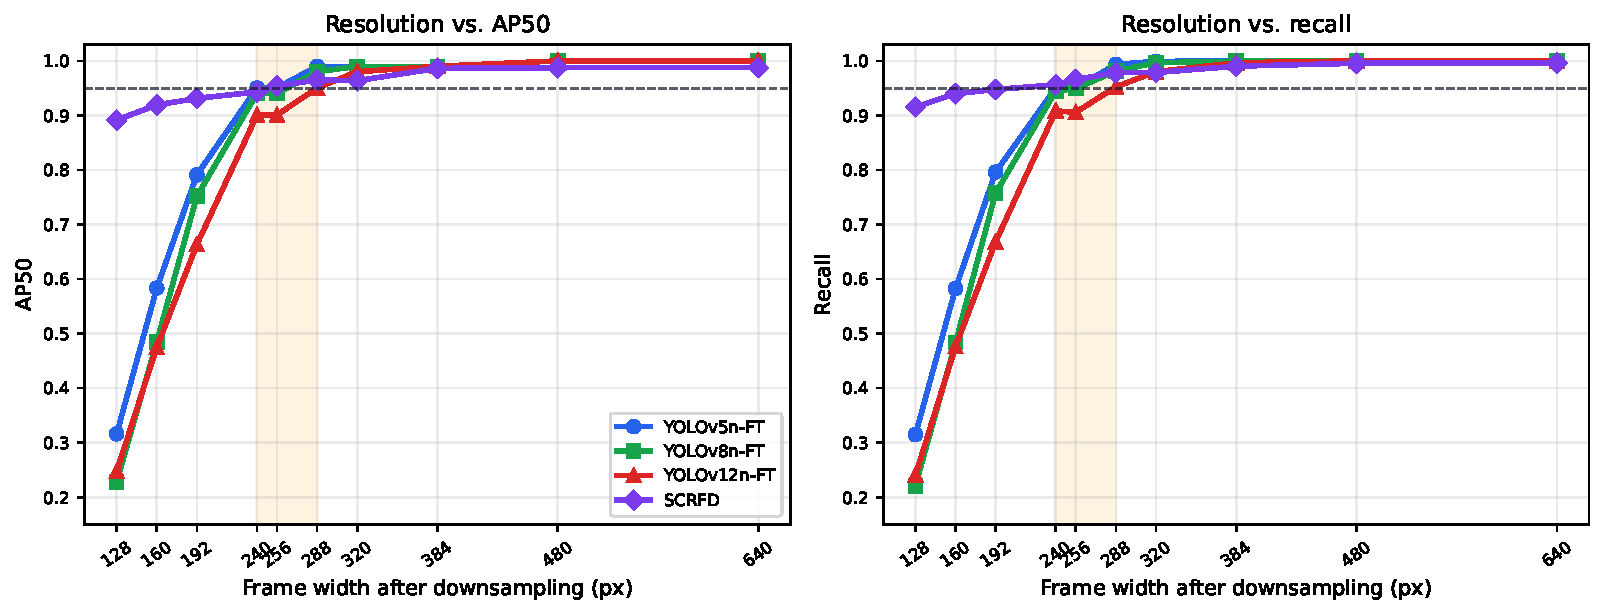
\includegraphics[width=0.95\textwidth]{chokepoint_data/modeling/ieee_paper_figures_en/fig01_accuracy_recall_vs_resolution.pdf}
\caption{AP$_{50}$ and recall as frame width is reduced at confidence 0.25.}
\label{fig:resolution}
\end{figure*}

\begin{figure*}[htbp]
\centering
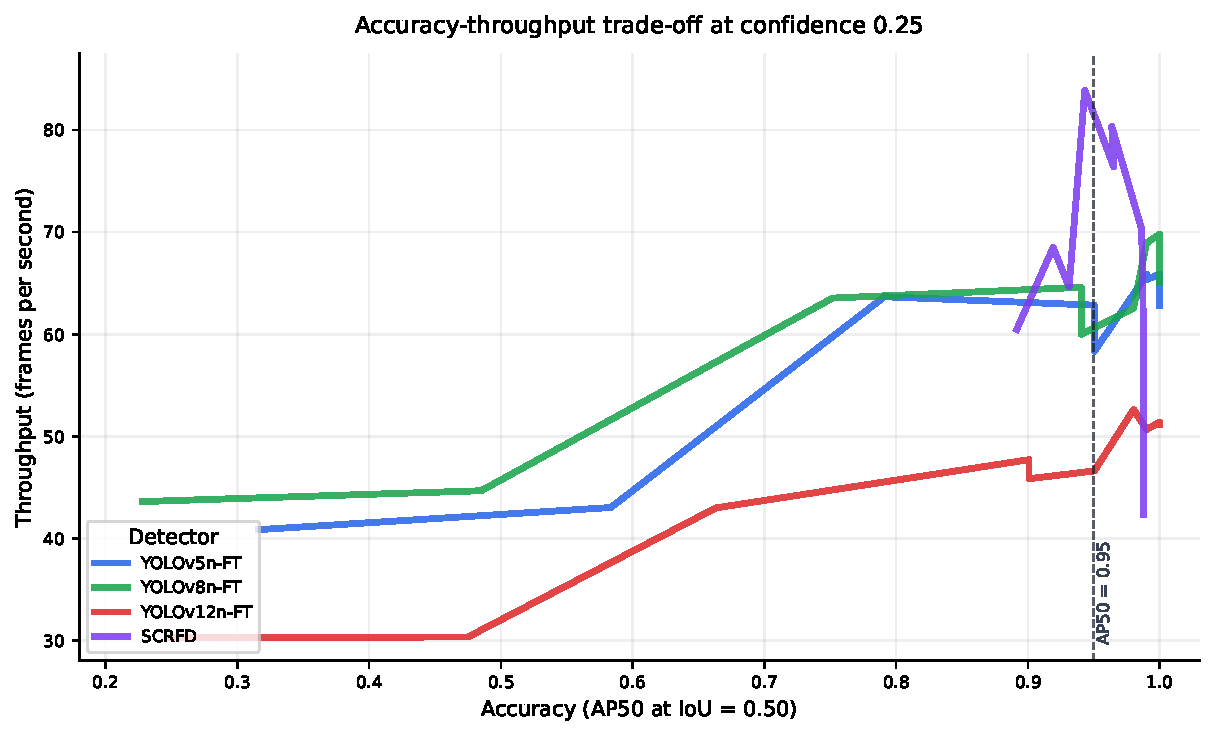
\includegraphics[width=0.85\textwidth]{chokepoint_data/modeling/ieee_paper_figures_en/fig02_accuracy_fps_tradeoff.pdf}
\caption{Accuracy-throughput trade-off. The horizontal axis is AP$_{50}$ and the vertical axis is frames per second.}
\label{fig:tradeoff}
\end{figure*}

\begin{figure*}[htbp]
\centering
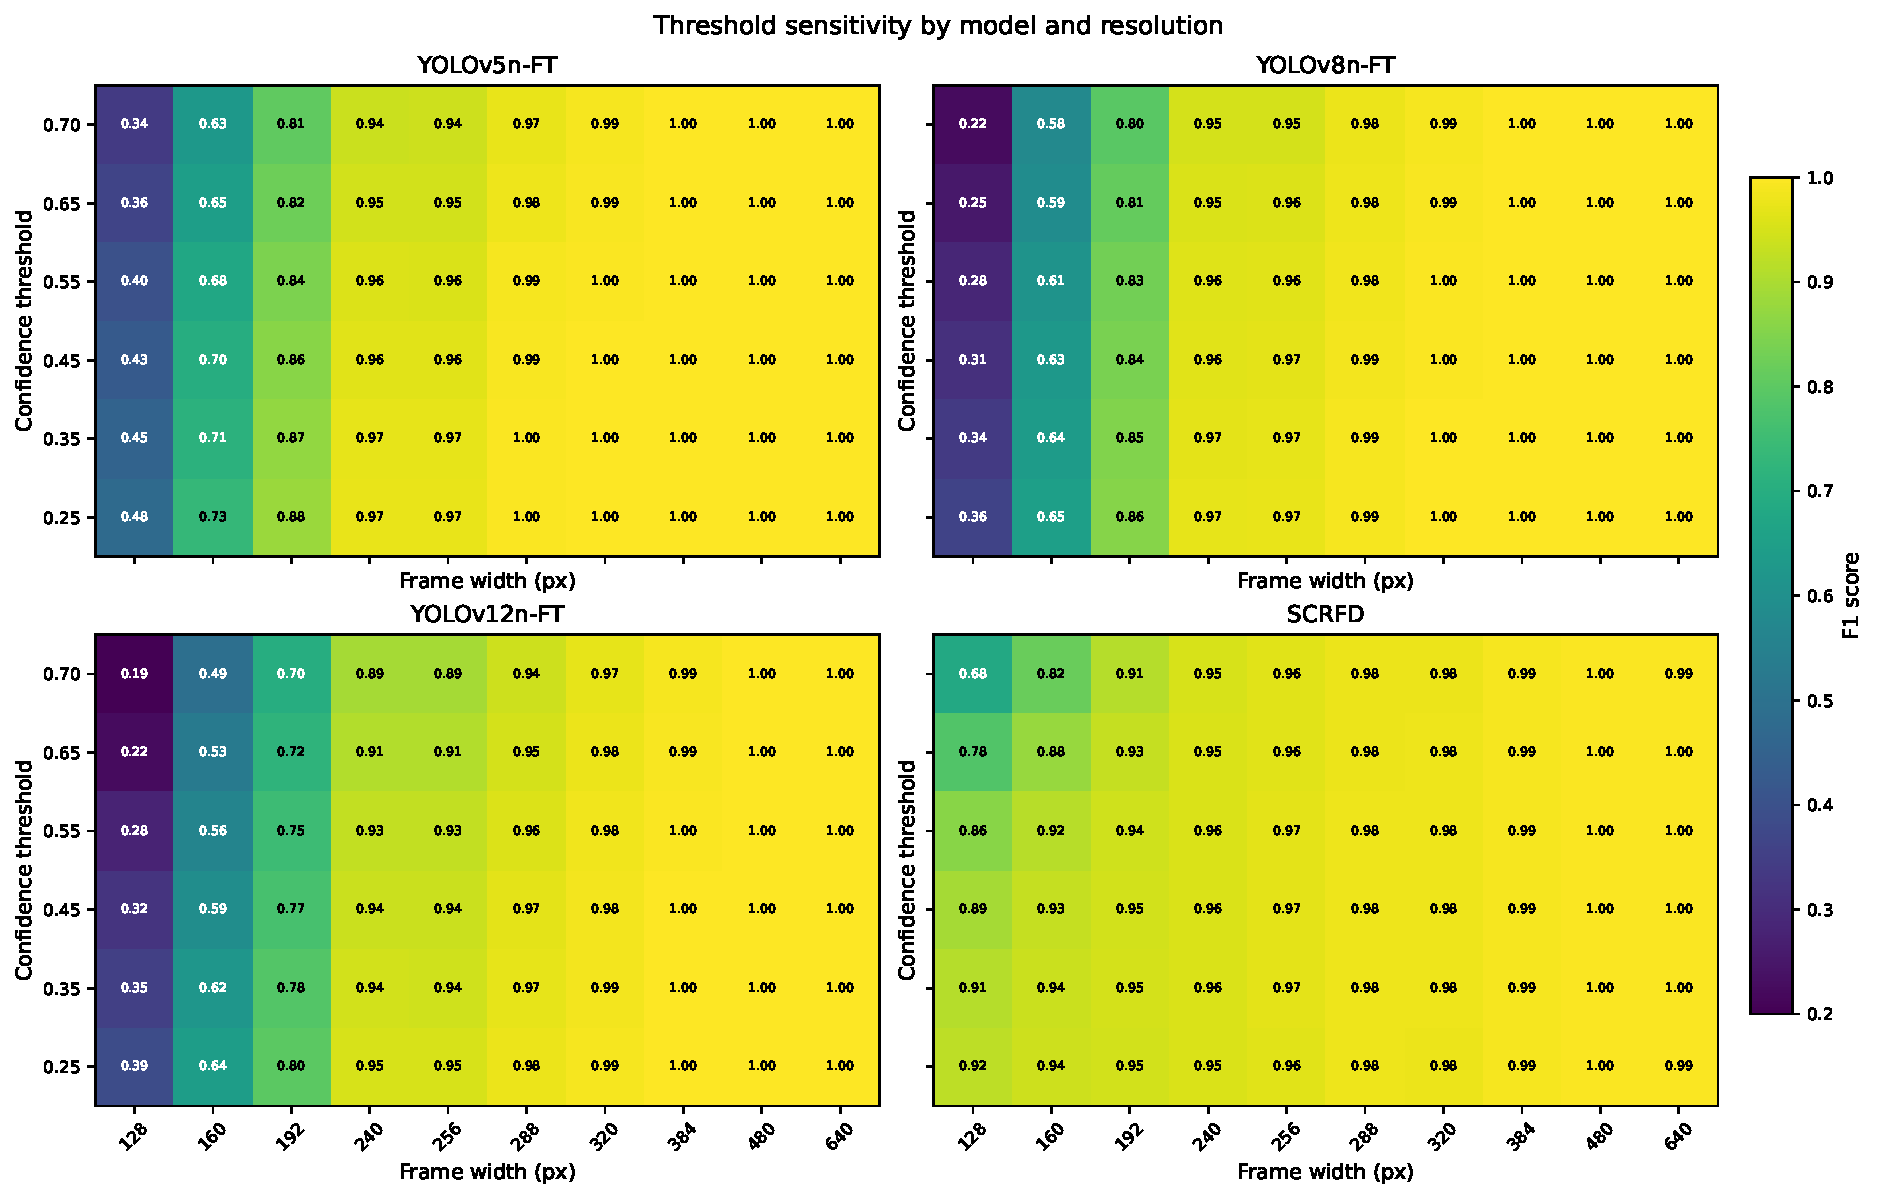
\includegraphics[width=0.95\textwidth]{chokepoint_data/modeling/ieee_paper_figures_en/fig03_threshold_f1_heatmap.pdf}
\caption{F1 sensitivity to confidence threshold and resolution.}
\label{fig:threshold}
\end{figure*}

\begin{figure*}[htbp]
\centering
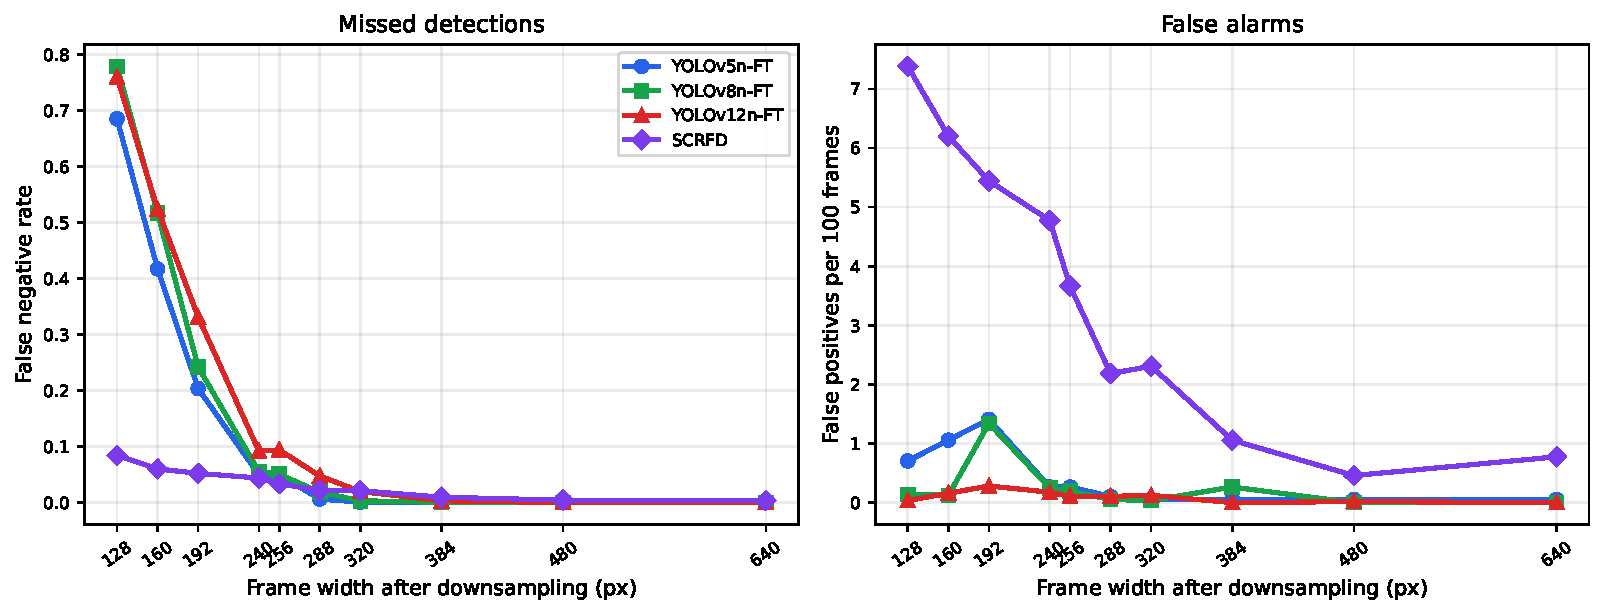
\includegraphics[width=0.95\textwidth]{chokepoint_data/modeling/ieee_paper_figures_en/fig04_error_modes_vs_resolution.pdf}
\caption{False negative and false positive behavior as resolution changes.}
\label{fig:error}
\end{figure*}

\begin{table}[htbp]
\caption{Smallest resolution satisfying AP$_{50}\geq0.95$ and recall $\geq0.95$.}
\label{tab:cutoff}
\centering
\begin{tabular}{lrrrr}
\toprule
Detector & Width & AP50 & Recall & FPS \\
\midrule
YOLOv5n-FT & 240 & 0.950 & 0.950 & 62.8 \\
YOLOv8n-FT & 288 & 0.980 & 0.981 & 62.5 \\
YOLOv12n-FT & 288 & 0.950 & 0.952 & 46.6 \\
SCRFD & 256 & 0.954 & 0.966 & 80.2 \\
\bottomrule
\end{tabular}
\end{table}

\section{Deployment Recommendations}
For favorable conditions where accuracy is the priority and GPU throughput is available, YOLOv8n-FT at 480$\times$360 or 640$\times$480 is recommended. It preserves AP$_{50}=1.000$ while running faster than YOLOv5n-FT and YOLOv12n-FT in the full-resolution evaluation. For constrained but reliable operation, YOLOv8n-FT at 288$\times$216 or 320$\times$240 is the most balanced choice. If the system must use the smallest acceptable frame, YOLOv5n-FT at 240$\times$180 is viable but leaves less safety margin. For poor conditions or extreme downsampling, SCRFD is more stable, but it should be treated as a fallback rather than a recommended recognition setting below the AP$_{50}$ target.

\section{Discussion}
The most important result is that the optimal resolution is not simply the lowest or highest tested value. The useful region is a band where faces are still large enough for reliable localization and the detector is still fast enough to reduce recognition-pipeline pressure. In this protocol, that band is 240--288 px width.

YOLOv12n-FT performs worse than expected for this specific deployment problem. It reaches perfect AP$_{50}$ at high resolution, but it is slower than YOLOv5n-FT and YOLOv8n-FT and loses accuracy sharply under strong downsampling. This suggests that attention-centric design does not automatically translate into better small-face robustness after resolution collapse.

\section{Limitations and Future Work}
The first limitation is the label protocol. ChokePoint provides eye landmarks, not native detector boxes, so this paper evaluates against deterministically derived boxes. The second limitation is scope. The current benchmark intentionally focuses on Portal 1 indoor frontal sequences because they match the office-door security-camera motivation. Future work should extend the protocol to Portal 2, crowded sequences, cross-camera transfer, and end-to-end recognition accuracy after detection.

\section{Conclusion}
This paper presented a ChokePoint-only benchmark for selecting the minimum useful resolution for lightweight face detection in surveillance video. The results show that 240--288 px frame width is the practical operating band for preserving detection quality while improving throughput. YOLOv8n-FT is the strongest balanced recommendation, YOLOv5n-FT provides the smallest acceptable resolution at 240$\times$180, and SCRFD remains the most robust fallback under extremely low resolution.

\begin{thebibliography}{00}
\bibitem{viola2004robust} P. Viola and M. J. Jones, ``Robust real-time face detection,'' \textit{Int. J. Comput. Vis.}, vol. 57, no. 2, pp. 137--154, 2004.
\bibitem{li2018lowreswild} P. Li, L. Prieto, D. Mery, and P. J. Flynn, ``On low-resolution face recognition in the wild: Comparisons and new techniques,'' arXiv:1805.11529, 2018.
\bibitem{redmon2016yolo} J. Redmon, S. Divvala, R. Girshick, and A. Farhadi, ``You Only Look Once: Unified, real-time object detection,'' in \textit{Proc. IEEE Conf. Comput. Vis. Pattern Recognit.}, 2016, pp. 779--788.
\bibitem{jocher2020yolov5} G. Jocher et al., ``ultralytics/yolov5,'' GitHub repository and software release, 2020--2022.
\bibitem{reis2023yolov8} D. Reis, J. Kupec, J. Hong, and A. Daoudi, ``Real-time flying object detection with YOLOv8,'' arXiv:2305.09972, 2023.
\bibitem{tian2025yolov12} Y. Tian, Q. Ye, and D. Doermann, ``YOLOv12: Attention-centric real-time object detectors,'' arXiv:2502.12524, 2025.
\bibitem{guo2021scrfd} J. Guo, J. Deng, A. Lattas, and S. Zafeiriou, ``Sample and computation redistribution for efficient face detection,'' arXiv:2105.04714, 2021.
\bibitem{wong2011chokepoint} Y. Wong, S. Chen, S. Mau, C. Sanderson, and B. C. Lovell, ``Patch-based probabilistic image quality assessment for face selection and improved video-based face recognition,'' in \textit{Proc. IEEE Biometrics Workshop, CVPR Workshops}, 2011, pp. 81--88.
\end{thebibliography}

\end{document}
